


\begin{frame}{Private Reader}

\vspace{1em}
\begin{figure}
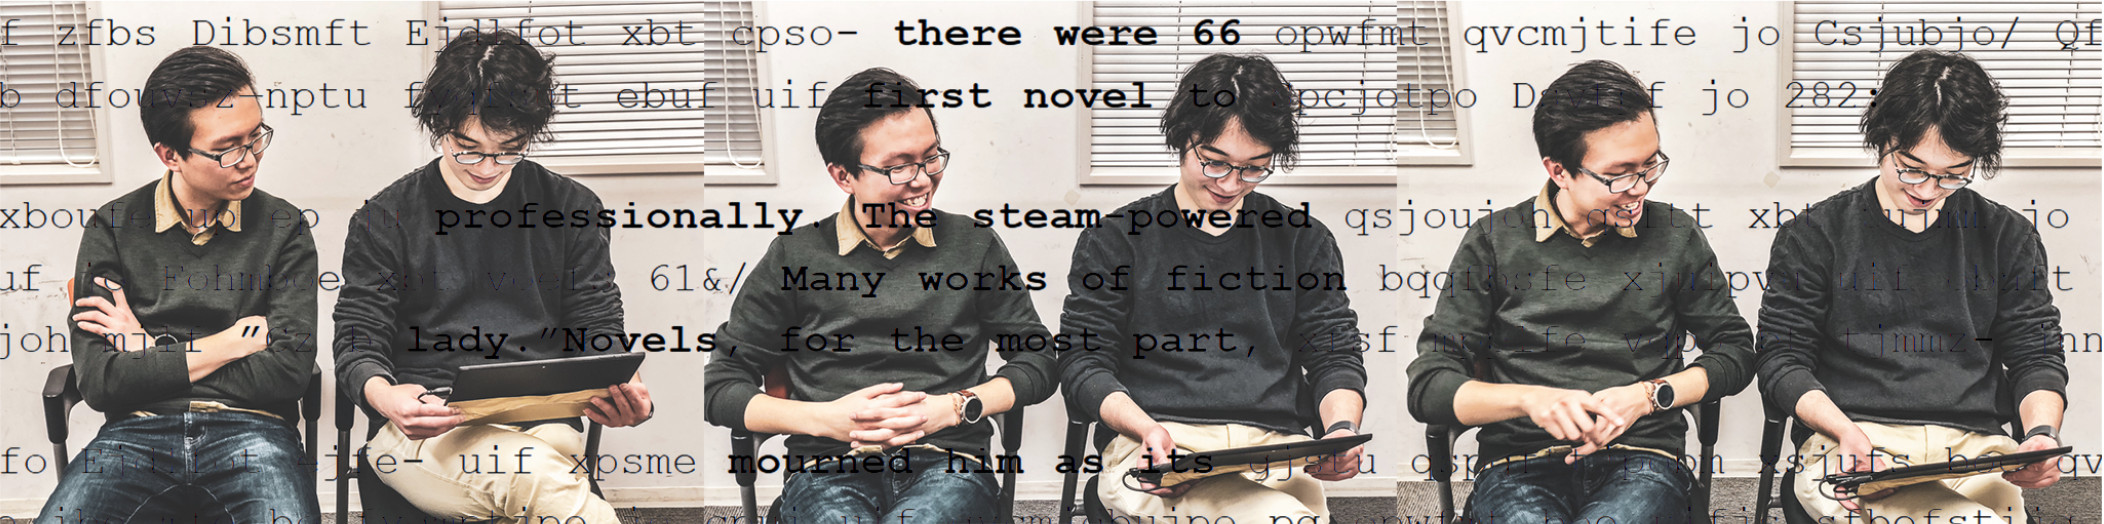
\includegraphics[width=\linewidth]{side/shouldersurfing.jpg}

\vspace{-1em}
\caption{\scriptsize The Private Reader Concept: Using eyetracking to make 
successful ``Shoulder Surfing'' more difficult.~\cite{Ragozin2019}.}
\end{figure}

\justifying

In a casual conversation with {\bf Prof. Kai Kunze} from Keio University (Japan)
we developed the idea that we could use {\bf eye tracking on mobile devices} to 
make ``shoulder surfing'' more difficult and thus enhance the privacy in
crowded, public spaces.

\vspace{1em}
The main idea consists in {\bf obfuscating the screen content} in those areas, 
{\bf where the user is currently not looking}. 

\vspace{1em}
In~\cite{Ragozin2019} students of Prof. Kunze investigated the idea by 
implementing a prototype and conducting a pilot study.

\vspace{1em}

\begin{center}
\rule{2cm}{0.4pt}\\[0.5em]
\end{center}

\fc{Ragozin2019}{publications/2019-04/2019-04}

\end{frame}
